\documentclass{article}
\usepackage{gvv-book}
\usepackage{gvv}
\usepackage{amsmath}
\usepackage{amsfonts}
\usepackage{tikz}
\usepackage{setspace}
\usepackage{gensymb}
\usepackage[cmex10]{amsmath}
\usepackage{amsthm}
\usepackage{mathrsfs}
\usepackage{txfonts}
\usepackage{stfloats}
\usepackage{bm}
\usepackage{cite}
\usepackage{cases}
\usepackage{subfig}
\usepackage{longtable}
\usepackage{multirow}
\usepackage{enumitem}
\usepackage{mathtools}
\usepackage{tikz}
\usepackage{circuitikz}
\usepackage{verbatim}
\usepackage[breaklinks=true]{hyperref}
\usepackage{tkz-euclide}
\usepackage{listings}
\usepackage{color}    
\usepackage{array}    
\usepackage{longtable}
\usepackage{calc}     
\usepackage{multirow} 
\usepackage{hhline}   
\usepackage{ifthen}   
\usepackage{lscape}     
\usepackage{chngcntr}
\usepackage{graphicx}
\usepackage{float}
\usepackage{multicol}
\usepackage[a4paper, left = 1.5cm, right = 1.5cm]{geometry}

\begin{document}

\begin{center}
\large
    \textbf{GATE 2019 : AEROSPACE ENGINEERING}\\
    AI25BTECH11029 - Samyak Gondane
\end{center}

\textbf{General Aptitude (GA)}
\textbf{Q.1 - Q.5 carry one mark each.}

\begin{enumerate}[leftmargin=*]
\item The fishermen, \underline{\hspace{1.5cm}} the flood victims owed their lives, were rewarded by the government.
\begin{multicols}{4}
\begin{enumerate}
\item whom
\item to which
\item to whom
\item that
\end{enumerate}
\end{multicols}

\item Some students were not involved in the strike. If the above statement is true, which of the following conclusions is/are logically necessary?
\begin{enumerate}
\item Some who were involved in the strike were students.
\item No student was involved in the strike.
\item At least one student was involved in the strike.
\item Some who were not involved in the strike were students.
\end{enumerate}
\begin{multicols}{4}
\begin{enumerate}
\item 1 and 2
\item 3
\item 4
\item 2 and 3
\end{enumerate}
\end{multicols}

\item The radius as well as the height of a circular cone increases by 10\%. The percentage increase in its volume is \underline{\hspace{1.5cm}}.
\begin{multicols}{4}
\begin{enumerate}
\item 17.1
\item 21.0
\item 33.1
\item 72.8
\end{enumerate}
\end{multicols}

\item Five numbers 10, 7, 5, 4 and 2 are to be arranged in a sequence from left to right following the directions given below:
\begin{enumerate}
\item No two odd or even numbers are next to each other.
\item The second number from the left is exactly half of the left-most number.
\item The middle number is exactly twice the right-most number.
\end{enumerate}
Which is the second number from the right?
\begin{multicols}{4}
\begin{enumerate}
\item 2
\item 4
\item 7
\item 10
\end{enumerate}
\end{multicols}

\item Until Iran came along, India had never been \underline{\hspace{1.5cm}} in kabaddi.
\begin{multicols}{4}
\begin{enumerate}
\item defeated
\item defeating
\item defeat
\item defeatist
\end{enumerate}
\end{multicols}

\textbf{Q.6 - Q.10 carry two marks each.}

\item Since the last one year, after a 125 basis point reduction in repo rate by the Reserve Bank of India, banking institutions have been making a demand to reduce interest rates on small saving schemes. Finally, the government announced yesterday a reduction in interest rates on small saving schemes to bring them on par with fixed deposit interest rates.

Which one of the following statements can be inferred from the given passage?
\begin{enumerate}
\item Whenever the Reserve Bank of India reduces the repo rate, the interest rates on small saving schemes are also reduced.
\item Interest rates on small saving schemes are always maintained on par with fixed deposit interest rates.
\item The government sometimes takes into consideration the demands of banking institutions before reducing the interest rates on small saving schemes.
\item A reduction in interest rates on small saving schemes follow only after a reduction in repo rate by the Reserve Bank of India.
\end{enumerate}

\item In a country of 1400 million population, 70\% own mobile phones. Among the mobile phone owners, only 294 million access the Internet. Among these Internet users, only half buy goods from e-commerce portals. What is the percentage of these buyers in the country?
\begin{multicols}{4}
\begin{enumerate}
\item 10.50
\item 14.70
\item 15.00
\item 50.00
\end{enumerate}
\end{multicols}

\item The nomenclature of Hindustani music has changed over the centuries. Since the medieval period dhrupad styles were identified as baanis. Terms like gayaki and baaj were used to refer to vocal and instrumental styles, respectively. With the institutionalization of music education the term gharana became acceptable. Gharana originally referred to hereditary musicians from a particular lineage, including disciples and grand disciples.

Which one of the following pairings is NOT correct?
\begin{multicols}{4}
\begin{enumerate}
\item dhrupad, baani
\item gayaki, vocal
\item baaj, institution
\item gharana, lineage
\end{enumerate}
\end{multicols}

\item Two trains started at 7AM from the same point. The first train travelled north at a speed of 80km/h and the second train travelled south at a speed of 100 km/h. The time at which they were 540 km apart is \underline{\hspace{1.5cm}} AM.
\begin{multicols}{4}
\begin{enumerate}
\item 9
\item 10
\item 11
\item 11.30
\end{enumerate}
\end{multicols}

\item “I read somewhere that in ancient times the prestige of a kingdom depended upon the number of taxes that it was able to levy on its people. It was very much like the prestige of a head-hunter in his own community.”

Based on the paragraph above, the prestige of a head-hunter depended upon
\begin{multicols}{2}
\begin{enumerate}
\item the prestige of the kingdom
\item the prestige of the heads
\item the number of taxes he could levy
\item the number of heads he could gather
\end{enumerate}
\end{multicols}
\end{enumerate}

\textbf{Aerospace Engineering (AE)}
\textbf{Q.1 - Q.25 carry one mark each.}

\begin{enumerate}[leftmargin=*, resume]
\item The maximum value of the function \( f(x) = xe^{-x} \) (where \( x \) is real) is
\begin{multicols}{4}
\begin{enumerate}
\item \( 1/e \)
\item \( 2/e^2 \)
\item \( (e^{-1/2})/2 \)
\item ∞
\end{enumerate}
\end{multicols}

\item Vector \( \vec{b} \) is obtained by rotating \( \vec{a} = \hat{i} + \hat{j} \) by 90° about \( \hat{k} \), where \( \hat{i}, \hat{j} \) and \( \hat{k} \) are unit vectors along the \( x, y \) and \( z \) axes, respectively. \( \vec{b} \) is given by
\begin{multicols}{4}
\begin{enumerate}
\item \( \hat{i} - \hat{j} \)
\item \( -\hat{i} + \hat{j} \)
\item \( \hat{i} + \hat{j} \)
\item \( -\hat{i} - \hat{j} \)
\end{enumerate}
\end{multicols}

\item A scalar function is given by \( f(x, y) = x^2 + y^2 \). Take \( \hat{i} \) and \( \hat{j} \) as unit vectors along the \( x \) and \( y \) axes, respectively. At \( (x, y) = (3, 4) \), the direction along which \( f \) increases the fastest is
\begin{multicols}{4}
\begin{enumerate}
\item \( \frac{1}{5}(4\hat{i} - 3\hat{j}) \)
\item \( \frac{1}{5}(3\hat{i} - 4\hat{j}) \)
\item \( \frac{1}{5}(3\hat{i} + 4\hat{j}) \)
\item \( \frac{1}{5}(4\hat{i} + 3\hat{j}) \)
\end{enumerate}
\end{multicols}

\item The dimensions of kinematic viscosity of a fluid (where \( L \) is length, \( T \) is time) are
\begin{multicols}{4}
\begin{enumerate}
\item \( LT^{-1} \)
\item \( LT^{-1} \)
\item \( LT^{-2} \)
\item \( LT^{-2}T \)
\end{enumerate}
\end{multicols}

\item \( \phi(x, y) \) represents the velocity potential of a two-dimensional flow with velocity field \( \vec{V} = u(x, y) \hat{i} + v(x, y)\hat{j} \), where \( \hat{i} \) and \( \hat{j} \) are unit vectors along the \( x \) and \( y \) axes, respectively. Which of the following is necessarily true?
\begin{multicols}{2}
\begin{enumerate}
\item \( \nabla^2 \phi = 0 \)
\item \( \nabla \times \vec{V} = 0 \)
\item \( \nabla \cdot \vec{V} = 0 \)
\item \( u = -\partial \phi / \partial y,  v = \partial \phi / \partial x \)
\end{enumerate}
\end{multicols}

\item For a quasi-one-dimensional isentropic supersonic flow through a diverging duct, which of the following is true in the direction of the flow?
\begin{enumerate}
\item Both the Mach number and the static temperature increase.
\item The Mach number increases and the static temperature decreases.
\item The Mach number decreases and the static temperature increases.
\item Both the Mach number and the static temperature decrease.
\end{enumerate}

\item For a NACA2415 airfoil of chord length \( c \), which of the following is true?
\begin{enumerate}
\item Maximum camber is located at 0.2\( c \) from the leading edge.
\item Maximum thickness is located at 0.15\( c \) from the leading edge.
\item Maximum camber is 0.02\( c \).
\item Maximum thickness is 0.05\( c \).
\end{enumerate}

\item When a propeller airplane in ground-roll during take-off experiences headwind, which of the following statement is \textbf{FALSE}?
\begin{multicols}{2}
\begin{enumerate}
    \item The drag on the airplane increases.
    \item The thrust from the propellers decreases.
    \item The wing lift increases.
    \item The ground-roll distance increases.

 
\end{enumerate}
\end{multicols}

\item For a single stage subsonic compressor, which of the following statements about the highest possible compressor pressure ratio (CPR) is correct?
\begin{enumerate}
\item CPR of an axial compressor > CPR of centrifugal compressor.
\item CPR of an axial compressor < CPR of centrifugal compressor.
\item CPR of an axial compressor = CPR of centrifugal compressor.
\item CPR of any value can be attained with either an axial or a centrifugal compressor.
\end{enumerate}

\item For a beam subjected to a transverse shear load through its shear center,
\begin{multicols}{2}
\begin{enumerate}
\item the twist per unit length is zero.
\item the shear stress is uniform throughout the cross-section.
\item the bending stresses in the cross section are zero.
\item the shear strain is zero at the shear center.
\end{enumerate}
\end{multicols}

\item A function \( f(x) \) is defined by \( f(x) = \frac{1}{2} (x + |x|) \). The value of
\[
\int_{-1}^{1} f(x)  dx
\]
is \underline{\hspace{1.5cm}} (round off to 1 decimal place).

\item The value of the following limit is \underline{\hspace{1.5cm}} (round off to 2 decimal places).
\[
\lim_{\theta \to 0} \frac{\theta - \sin \theta}{\theta^3}
\]

\item To simulate the aerodynamic forces on a cylinder of 1 m diameter due to a uniform air flow of 1 m/s at standard temperature and pressure (STP), low-speed wind tunnel experiments at STP are conducted on a 0.1 m diameter cylinder. The free stream air speed in the wind tunnel experiments should be \underline{\hspace{1.5cm}} m/s (round off to the nearest integer).

\item The power-off glide range for an airplane with a maximum Lift to Drag ratio of 18, when the glide starts at an altitude of 4 km, is \underline{\hspace{1.5cm}} km (round off to the nearest integer).

\item For an airplane flying in a vertical plane, the angle of attack is 3°, the horizontal and vertical components of velocity in wind axis are 300 km/h and 15.72 km/h, respectively. The pitch attitude of the airplane is \underline{\hspace{1.5cm}} degrees (round off to 2 decimal places).

\item An airplane is in steady level flight with a true air speed of 50 m/s. The ambient air density and ambient pressure at the flight altitude are 0.91 kg/m\(^3\) and 7×10\(^4\) N/m\(^2\), respectively. At sea level, air density is 1.225 kg/m\(^3\) and ambient pressure is 1.01×10\(^5\) N/m\(^2\). The equivalent or indicated air speed of the airplane is \underline{\hspace{1.5cm}} m/s (round off to 2 decimal places).

\item For the complete combustion of 1 mole of ethanol (C₂H₅OH), the required number of moles of oxygen is \underline{\hspace{1.5cm}}.

\item One kg of diatomic gas is heated and its temperature increases from 100 K to 600 K. The energy added at constant pressure during this process is 500 kJ. The specific heat at constant volume for the gas is \underline{\hspace{1.5cm}} kJ/kgK (round off to 2 decimal places).

\item The number of independent elastic constants for a homogeneous isotropic linear elastic material is \underline{\hspace{1.5cm}}.

\item A thin plate with Young’s modulus 210 GPa and Poisson’s ratio 0.3 is loaded as shown in the figure. The change in length along the y-direction is \underline{\hspace{1.5cm}} mm (round off to 1 decimal place).
\begin{figure}[H]
    \centering
    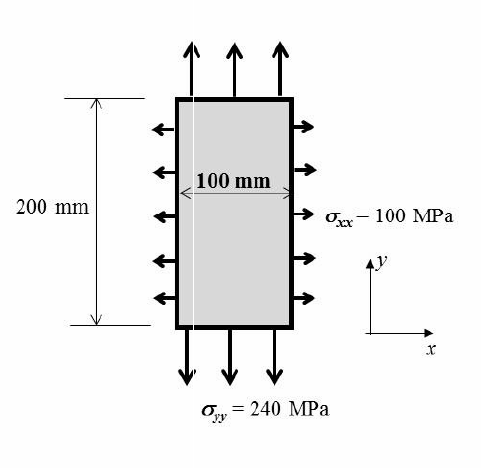
\includegraphics[width=0.3\linewidth]{figs/q30.png}
    \caption{}
    \label{fig:q30}
\end{figure}

\item For the state of stress shown in the figure, the normal stress, \(\sigma_n\), on a plane inclined at 45 degrees to the x-axis is \underline{\hspace{1.5cm}} MPa (round off to the nearest integer).
\begin{figure}[H]
    \centering
    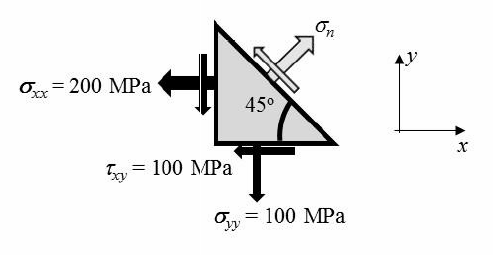
\includegraphics[width=0.3\linewidth]{figs/q31.png}
    \caption{}
    \label{fig:q31}
\end{figure}

\item In the spring-mass system, shown in the figure, mass \( m = 3 \) kg and the spring stiffness \( k = 20 \) kN/m. The natural frequency of the system is \underline{\hspace{1.5cm}} Hz (round off to the nearest integer).
\begin{figure}[H]
    \centering
    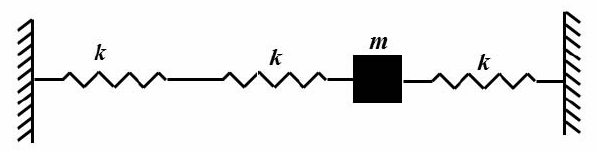
\includegraphics[width=0.3\linewidth]{figs/q32.png}
    \caption{}
    \label{fig:q32}
\end{figure}

\textbf{Q.26 - Q.55 carry two marks each.}

\item The following system of equations
\begin{align}
    2x - y - z = 0,\\
-x + 2y - z = 0,\\
-x - y + 2z = 0
\end{align}

\begin{multicols}{4}
\begin{enumerate}
\item has no solution.
\item has a unique solution.
\item has three solutions.
\item has an infinite number of solutions.
\end{enumerate}
\end{multicols}

\item A supersonic flow in a constant area duct at Mach number \( M_1 \) encounters a ramp of angle \(\theta_1\) (see Figure 1). The resulting oblique shock with shock angle \(\beta_1\) is then reflected from the top wall. For the reflected shock, the turn angle is \(\theta_2\) and the shock angle is \(\beta_2\).
\begin{figure}[H]
    \centering
    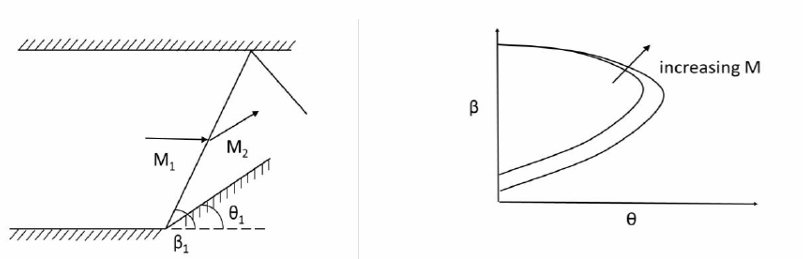
\includegraphics[width=0.3\linewidth]{figs/q34.png}
    \caption{}
    \label{fig:q34}
\end{figure}

Use the weak shock solution from the \(\theta\)-\(\beta\)-M plot shown in Figure 2 to choose the correct option from the following.
\begin{multicols}{4}
\begin{enumerate}
\item \(\beta_1 > \beta_2\)
\item \(\beta_1 < \beta_2\)
\item \(\theta_1 > \theta_2\)
\item \(\theta_1 < \theta_2\)
\end{enumerate}
\end{multicols}

\item Which of the following statements about adverse yaw of an airplane is/are correct?
\begin{enumerate}
\item P. It is caused by flow separation resulting from large rudder deflection.
\item Q. It is caused by dissimilar drag forces acting on the two halves of the wing resulting from aileron deflections of same magnitude.
\item R. It can be eliminated by ensuring that the upward deflection of one aileron is greater than the downward deflection of the opposite aileron.
\end{enumerate}
\begin{multicols}{4}
\begin{enumerate}
\item P only
\item Q only
\item P and R
\item Q and R
\end{enumerate}
\end{multicols}

\item In a turbojet engine, the compressor outlet temperature increases with decreasing efficiency of the compressor. If the turbine inlet temperature remains constant, with decreasing efficiency of the compressor, the thrust specific fuel consumption of the engine
\begin{multicols}{2}
\begin{enumerate}
\item decreases, as the heat input is lower.
\item remains unchanged.
\item increases, as the compressor needs more work input from the turbine.
\item decreases, as the thrust produced is higher.
\end{enumerate}
\end{multicols}

\item For a 1 m long simply supported beam with a concentrated vertical load of 200 N and a concentrated bending moment of 100 Nm at the center as shown in the figure, the correct bending moment diagram is:
\begin{figure}[H]
    \centering
    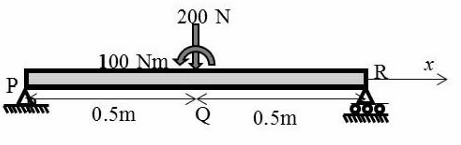
\includegraphics[width=0.5\linewidth]{figs/q37.png}
    \caption{}
    \label{fig:q37}
\end{figure}
\begin{enumerate}
\item \begin{figure}[H]
    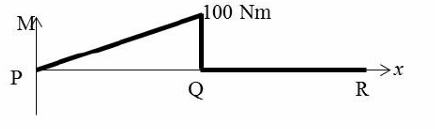
\includegraphics[width=0.3\linewidth]{figs/q37(a).png}
    \caption{}
    \label{fig:q37(a)}
\end{figure}
\item \begin{figure}[H]
    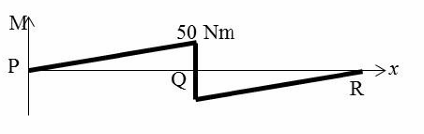
\includegraphics[width=0.3\linewidth]{figs/q37(b).png}
    \caption{}
    \label{fig:q37(b)}
\end{figure}
\item \begin{figure}[H]
    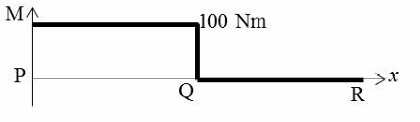
\includegraphics[width=0.3\linewidth]{figs/q37(c).png}
    \caption{}
    \label{fig:q37(c)}
\end{figure}
\item \begin{figure}[H]
    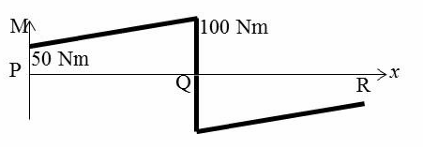
\includegraphics[width=0.3\linewidth]{figs/q37(d).png}
    \caption{}
    \label{fig:q37(d)}
\end{figure}
\end{enumerate}

\item For real \( x \), the number of points of intersection between the curves \( y = x \) and \( y = \cos x \) is \underline{\hspace{1.5cm}}.

\item One of the eigenvalues of the following matrix is 1.
\myvec{x & 2 \\
-1 & 3}

The other eigenvalue is \underline{\hspace{1.5cm}}.

\item The curve \( y = f(x) \) is such that its slope is equal to \( y^2 \) for all real \( x \). If the curve passes through (1, -1), the value of \( y \) at \( x = -2 \) is \underline{\hspace{1.5cm}} (round off to 1 decimal place).

\item The inviscid, incompressible flow field resulting from a uniform flow past a circular cylinder of radius \( R \) centered at the origin is given by:
\[
u_r = U \left( 1 - \frac{R^2}{r^2} \right) \cos \theta \quad u_\theta = -U \left( 1 + \frac{R^2}{r^2} \right) \sin \theta
\]
\begin{figure}[H]
    \centering
    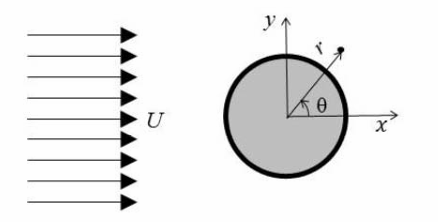
\includegraphics[width=0.3\linewidth]{figs/q41.png}
    \caption{}
    \label{fig:q41}
\end{figure}
where \( u_r \) and \( u_\theta \) are the radial and azimuthal velocity components in polar coordinates, (\( r, \theta \)), as shown in the figure. \( U \) is the free stream speed. Ignore the effects of gravity. The azimuthal location (in the first quadrant) on the cylinder at which the pressure coefficient is zero is \underline{\hspace{1.5cm}} degrees (round off to the nearest integer).

\item A cylindrical container of radius \( R = 50  \text{cm} \) is filled with water up to a height \( h_0 \). Upon rotating the cylinder about its central axis at a constant angular speed, the free surface takes a parabolic shape (see figure), and is displaced upwards by \( h_1 = 10  \text{cm} \) at \( r = R \). The magnitude of the downward displacement \( h_2 \) of the free surface at \( r = 0 \) is \underline{\hspace{1.5cm}} cm (round off to the nearest integer).
\begin{figure}[H]
    \centering
    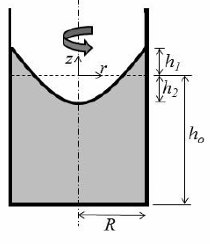
\includegraphics[width=0.2\linewidth]{figs/q42.png}
    \caption{}
    \label{fig:q42}
\end{figure}

\item A two-dimensional, incompressible fluid flow is described by the stream function \( \Psi = xy^3  \text{m}^2/\text{s} \) on the Cartesian x-y plane. If the density and dynamic viscosity of the fluid are 1 kg/m\(^3\) and 0.1 kg/m-s, respectively, the magnitude of the pressure gradient in the \( x \) direction at \( x=1  m \) and \( y=1  m \) is \underline{\hspace{1.5cm}} N/m\(^3\) (round off to 1 decimal place).

\item The static pressure ratio across a stationary normal shock is given by
\[
\frac{p_2}{p_1} = 1 + \frac{2\gamma}{\gamma + 1} (M_1^2 - 1),
\]
where \( M_1 \) is the upstream Mach number. For a stationary normal shock in air (\(\gamma = 1.4, R = 287  J/kg-K\)) with upstream flow conditions given by: speed 800 m/s, static temperature 300 K and static pressure 1 atm., the static pressure downstream of the shock is \underline{\hspace{1.5cm}} atm. (round off to 2 decimal places).

\item For a symmetric airfoil at an angle of attack of \(10^\circ\), assuming thin airfoil theory, the magnitude of the pitching moment coefficient about the leading edge is \underline{\hspace{1.5cm}} (round off to 2 decimal places).

\item The span-wise distribution of circulation over a finite wing of span \(b = 10  \text{m}\) is
\[
\Gamma(y) = \Gamma_0 \sqrt{1 - \left( \frac{2y}{b} \right)^2}
\]
If \(\Gamma_0 = 20  \text{m}^2/\text{s}\) and the free stream density and speed are 1.2 kg/m\(^3\) and 100 m/s, respectively, the total lift is \underline{\hspace{1.5cm}} kN (round off to 2 decimal places).

\item The airplane shown in figure starts executing a symmetric pull-up maneuver from steady level attitude with a constant nose-up pitch acceleration of 20 deg/s\(^2\). The vertical load factor measured at this instant at the centre of gravity (CG) is 2. Given that the acceleration due to gravity is 9.81 m/s\(^2\), the vertical load factor measured at point P on the nose of the airplane, which is 2 m ahead of the CG, is \underline{\hspace{1.5cm}} (round off to 2 decimal places).
\begin{figure}[H]
    \centering
    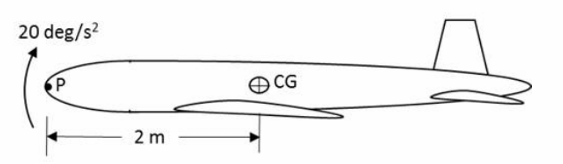
\includegraphics[width=0.4\linewidth]{figs/q47.png}
    \caption{}
    \label{fig:q47}
\end{figure}

\item Consider an airplane with a weight of 8000 N, wing area of 16 m\(^2\), wing zero-lift drag coefficient of 0.02, Oswald’s efficiency factor of 0.8, and wing aspect ratio of 6, in steady level flight with wing lift coefficient of 0.375. Considering the same flight speed and ambient density, the ratio of the induced drag coefficient during steady level flight to that during a \(30^\circ\) climb is \underline{\hspace{1.5cm}} (round off to 2 decimal places).

\item The product of earth’s mass (\(M\)) and the universal gravitational constant (\(G\)) is \(GM = 3.986 \times 10^{14}  \text{m}^3/\text{s}^2\). The radius of earth is 6371 km. The minimum increment in the velocity to be imparted to a spacecraft flying in a circular orbit around the earth at an altitude of 4000 km to make it exit earth’s gravitational field is \underline{\hspace{1.5cm}} km/s (round off to 2 decimal places).

\item A propeller driven airplane has a gross take-off weight of 4905 N with a wing area of 6.84 m\(^2\). Assume that the wings are operating at the maximum \(C_{L}^{3/2}/C_p\) of 13, the propeller efficiency is 0.9 and the specific fuel consumption of the engine is 0.76 kg/kW-hr. Given that the density of air at sea level is 1.225 kg/m\(^3\) and the acceleration due to gravity is 9.81 m/s\(^2\), the weight of the fuel required for an endurance of 18 hours at sea level is \underline{\hspace{1.5cm}} N (round off to the nearest integer).

\item The design of an airplane is modified to increase the vertical tail area by 20 percent and decrease the moment arm from the aerodynamic centre of the vertical tail to the airplane centre of gravity by 20 percent. Assuming all other factors remain unchanged, the ratio of the modified to the original directional static stability (\(C_{V_g}\) due to tail fin) is \underline{\hspace{1.5cm}} (round off to 2 decimal places).

\item For a rocket engine, the velocity ratio \(r\) is \(V_a/V_s\), where \(V_a\) is the vehicle velocity and \(V_s\) is the exit velocity of the exhaust gases. Assume the flow to be optimally expanded through the nozzle. For \(r = 2\), if \(F\) is the thrust produced and \(\dot{m}\) is the mass flow rate of exhaust gases, then, \(F/(\dot{m}V_a)\) is \underline{\hspace{1.5cm}}.

\item The specific impulse of a rocket engine is 3000 Ns/kg. The mass of the rocket at burnout is 1000 kg. The propellant consumed in the process is 720 kg. Assume all factors contributing to velocity loss to be negligible. The change in vehicle velocity \(\Delta u\) is \underline{\hspace{1.5cm}} km/s (round off to 2 decimal places).

\item The combustion products of a gas turbine engine can be assumed to be a calorically perfect gas with \(\gamma = 1.2\). The pressure ratio across the turbine stage is 0.14. The measured turbine inlet and exit stagnation temperatures are 1200 K and 900 K, respectively. The total-to-total turbine efficiency is \underline{\hspace{1.5cm}} \% (round off to the nearest integer).

\item The figure shows the velocity triangles for an axial compressor stage. The specific work input to the compressor stage is \underline{\hspace{1.5cm}} kJ/kg (round off to 2 decimal places).
\begin{figure}[H]
    \centering
    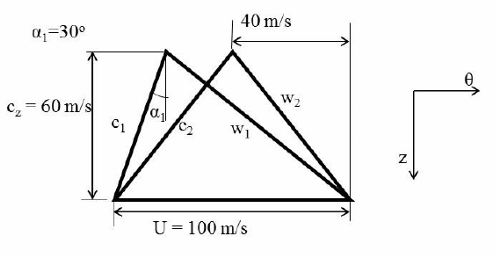
\includegraphics[width=0.4\linewidth]{figs/q55.png}
    \caption{}
    \label{fig:q55}
\end{figure}

\item As shown in the figure, a rigid slab CD of weight \( W \) (distributed uniformly along its length) is hung from a ceiling using three cables of identical length and cross-sectional area. The central cable is made of steel (Young’s modulus = 3E) and the other two cables are made of aluminium (Young’s modulus = E). The percentage of the total weight taken by the central cable is \underline{\hspace{1.5cm}} \% (round off to the nearest integer).
\begin{figure}[H]
    \centering
    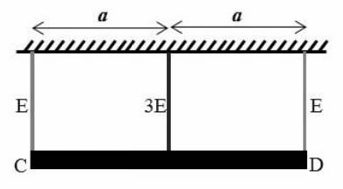
\includegraphics[width=0.3\linewidth]{figs/q56.png}
    \caption{}
    \label{fig:q56}
\end{figure}

\item All the bars in the given truss are elastic with Young’s modulus 200 GPa, and have identical cross-sections with moment of inertia 0.1 cm\(^4\). The lowest value of the load \( P \) at which the truss fails due to buckling is \underline{\hspace{1.5cm}} kN (round off to the nearest integer).
\begin{figure}[H]
    \centering
    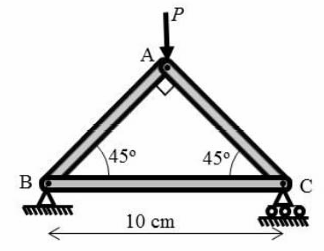
\includegraphics[width=0.3\linewidth]{figs/q57.png}
    \caption{}
    \label{fig:q57}
\end{figure}

\item A solid circular shaft is designed to transmit a torque \( T \) with a factor of safety of 2. It is proposed to replace the solid shaft by a hollow shaft of the same material and identical outer radius. If the inner radius is half the outer radius, the factor of safety for the hollow shaft is \underline{\hspace{1.5cm}} (round off to 1 decimal place).
\begin{figure}[H]
    \centering
    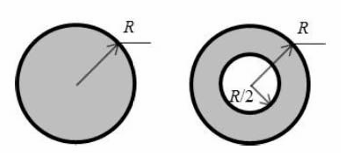
\includegraphics[width=0.3\linewidth]{figs/q58.png}
    \caption{}
    \label{fig:q58}
\end{figure}

\item In the structure shown in the figure, bars AB and BC are made of identical material and have circular cross-sections of 10 mm radii. The yield stress of the material under uniaxial tension is 280 MPa. Using the von Mises yield criterion, the maximum load along the z-direction (perpendicular to the plane of paper) that can be applied at C, such that AB does not yield is \underline{\hspace{1.5cm}} N (round off to the nearest integer).
\begin{figure}[H]
    \centering
    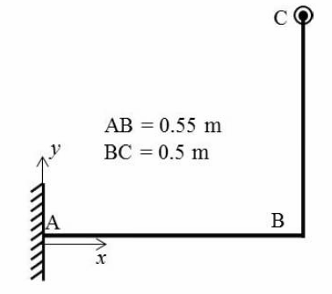
\includegraphics[width=0.3\linewidth]{figs/q59.png}
    \caption{}
    \label{fig:q59}
\end{figure}

\item A thin-walled tube, with the cross-section shown in the figure, is subjected to a torque of \( T = 1  \text{kN-m} \). The walls have uniform thickness \( t = 1  \text{mm} \) and shear modulus \( G = 26  \text{GPa} \). Assume that the curved portion is semi-circular. The shear stress in the wall is \underline{\hspace{1.5cm}} MPa (round off to 1 decimal place).
\begin{figure}[H]
    \centering
    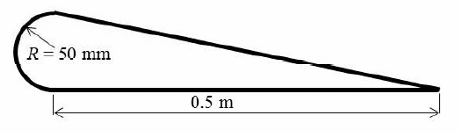
\includegraphics[width=0.3\linewidth]{figs/q60.png}
    \caption{}
    \label{fig:q60}
\end{figure}

\item For a damped spring-mass system, mass \( m = 10  \text{kg} \), stiffness \( k = 10^3  \text{N/m} \), and damping coefficient \( c = 20  \text{kg/s} \). The ratio of the amplitude of oscillation of the first cycle to that of the fifth cycle is \underline{\hspace{1.5cm}} (round off to 1 decimal place).

\item For the system of springs and masses shown below, \( k = 1250  \text{N/m} \) and \( m = 10  \text{kg} \). The highest natural frequency, \( \omega_1 \) of the system is \underline{\hspace{1.5cm}} radians/s (round off to the nearest integer).
\begin{figure}[H]
    \centering
    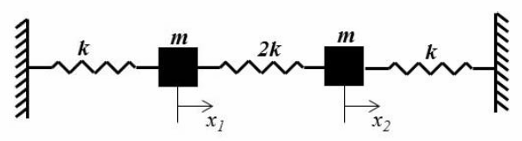
\includegraphics[width=0.3\linewidth]{figs/q62.png}
    \caption{}
    \label{fig:q62}
\end{figure}\\
\\
\centering
\large
\textbf{END OF THE QUESTION PAPER}

\end{enumerate}

\end{document}